%!TEX root = Slic3r-Manual.tex

\subsection{Sequential Printing} % (fold)
\label{sec:sequential_printing}
\index{Sequential Printing}

When printing several objects at once it can be useful to print each one separately as this will minimise oozing and strings running between the prints.  It will also decrease the risk of a problem ruining the entire print - if one part detaches or fails in some way, it will not be dragged into other parts of the print during each layer.

\begin{figure}[H]
\centering
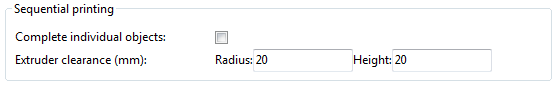
\includegraphics[keepaspectratio=true,width=1\textwidth]{simple_mode/sequential_printing_options.png}
\caption{Sequential printing options.}
\label{fig:sequential_printing_options}
\end{figure}

\index{Print Settings!Sequential printing!Extruder clearance}
Care has to be taken that the nozzle and extruder does not interfere with already printed parts.  Slic3r should warn if it detects the nozzle or extruder will collide with a part, but double check that the layout of the parts will not cause problems.  The \texttt{Extruder clearance} parameters help Slic3r detect potential collisions:
\begin{itemize}
	\item \texttt{Radius}  - The clearance that should be given around the extruder.  Take care if the extruder is not mounted centrally - take the largest safe value.
	\item \texttt{Height}  - The vertical distance between the nozzle tip and the X axis rods, or lowest part which may interfere with a finished print.
\end{itemize}

\begin{figure}[H]
\centering
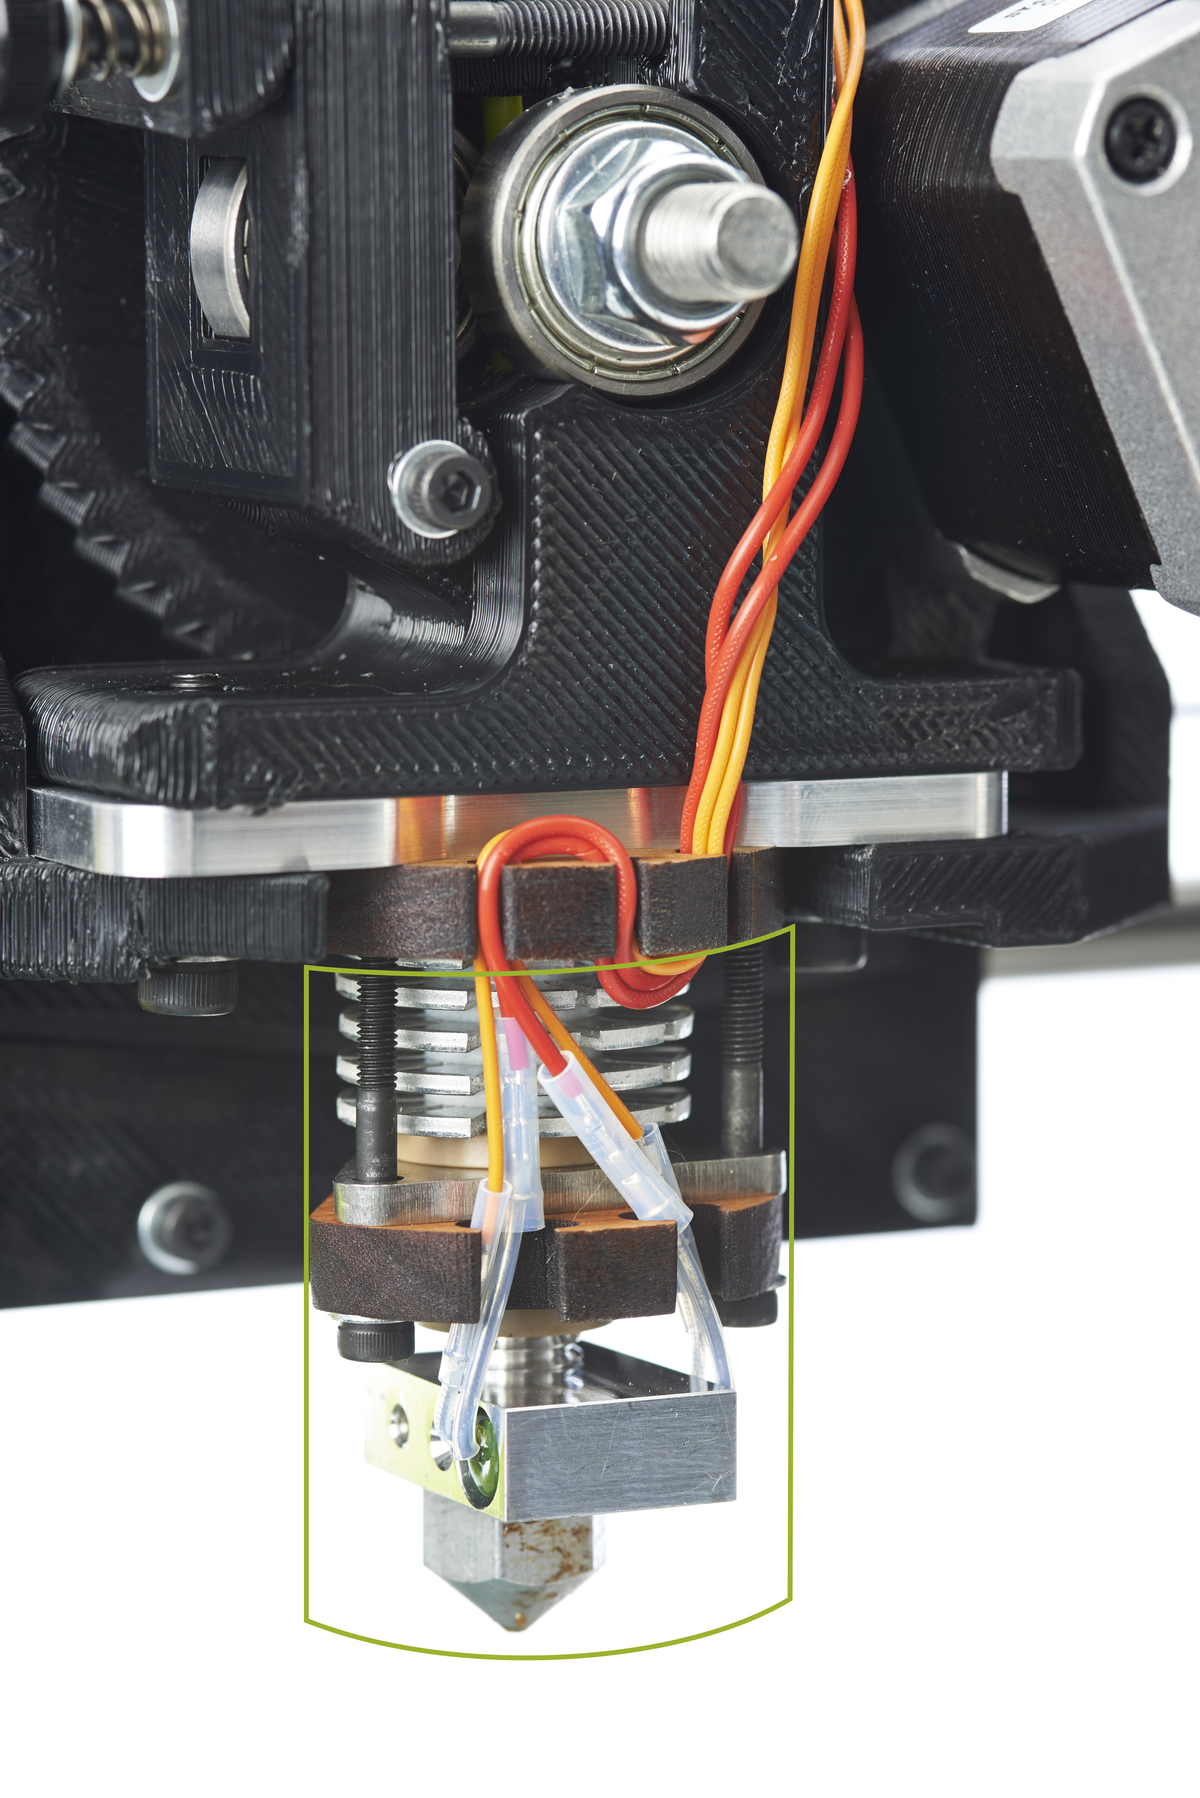
\includegraphics[keepaspectratio=true,width=0.5\textwidth]{simple_mode/extruder_clearance.jpg}
\caption{The clearance cylinder around an extruder.}
\label{fig:a_diagram_depicting_extruder_clearance}
\end{figure}

